% These are the lecture notes for my CSCI360 course SPRING 2017
% at John Jay College of Criminal Justice.

% Feel free to edit these slides and use them for your own courses.
% HOWEVER DO NOT REMOVE THESE LINES!
% Email me at: awood [at] jjay.cuny.edu
% or at: awood [at] gradcenter.cuny.edu


\documentclass{beamer}

\usepackage{tikz}
\usetikzlibrary{calc}

\usepackage{forest}
\usepackage{verbatim}
\usepackage{color}


\setbeamertemplate{footline}[frame number]
\setbeamertemplate{navigation symbols}{} 

\newtheorem{thm}{Theorem}[section]
\newtheorem{lem}{Lemma}
\newtheorem{cl}{Claim}
\newtheorem{cor}{Corollary}[section]
\newtheorem{conj}{Conjecture}
\newtheorem{quest}{Question}
\newtheorem{defn}{Definition}[section]
\newtheorem{obs}{Observation}[section]
\newtheorem{exam}{Example}

\newcommand{\im}{\operatorname{im}}
\newcommand{\id}{\operatorname{id}}
\newcommand{\interior}{\operatorname{int}}
\newcommand{\bdry}{\operatorname{bdry}}
\newcommand{\<}{\langle}
\renewcommand{\>}{\rangle}
\newcommand{\Gab}{(G_\phi)^{ab}} 
\newcommand{\phibar}{\bar{\phi}}
\newcommand{\Z}{\mathbb{Z}}
\newcommand{\N}{\mathbb{N}}
\newcommand{\Q}{\mathbb{Q}}
\newcommand{\R}{\mathbb{R}}
\newcommand{\C}{\mathbb{C}}
\newcommand{\A}{\mathcal{A}}
\newcommand{\OO}{\mathcal{O}}
\newcommand{\UU}{\mathcal{U}}
\newcommand{\power}{2^{\{P_1, \cdots , P_n\}}}
\newcommand{\bp}{\begin{problem}}
\newcommand{\ep}{\end{problem}}
\newcommand{\ba}{\begin{answer}}
\newcommand{\ea}{\end{answer}}
\newcommand{\ds}{\displaystyle}
\newcommand{\ben}{\renewcommand{\theenumi}{\alph{enumi}}
\renewcommand{\labelenumi}{(\theenumi)}\begin{enumerate}}
\newcommand{\een}{\end{enumerate}}
\newcommand{\Hess}{\operatorname{Hessian}}
\newcommand{\Aut}{\mathrm{Aut}}
\newcommand{\Inn}{\mathrm{Inn}}
\newcommand{\Out}{\mathrm{Out}}
\newcommand{\End}{\mathrm{End}}


\mode<presentation>
{
%  \usetheme{default}
  \setbeamercovered{invisible}
}


\usepackage[english]{babel}
\usepackage[latin1]{inputenc}
\usepackage{times}
\usepackage[T1]{fontenc}
\usepackage{stmaryrd}

%\usetheme{default}
%\usetheme{AnnArbor}
%\usetheme{Antibes}
%\usetheme{Bergen}
%\usetheme{Berkeley}
%\usetheme{Berlin}
%\usetheme{Boadilla}
%\usetheme{CambridgeUS}
%\usetheme{Copenhagen}
%\usetheme{Darmstadt}
%\usetheme{Dresden}
%\usetheme{Frankfurt}
%\usetheme{Goettingen}
%\usetheme{Hannover}
%\usetheme{Ilmenau}
%\usetheme{JuanLesPins}
%\usetheme{Luebeck}
%\usetheme{Madrid}
%\usetheme{Malmoe}
%\usetheme{Marburg}
%\usetheme{Montpellier}
%\usetheme{PaloAlto}
%\usetheme{Pittsburgh}
%\usetheme{Rochester}
\usetheme{Singapore}
%\usetheme{Szeged}
%\usetheme{Warsaw}

%\usecolortheme{default}
%\usecolortheme{albatross}
\usecolortheme{beaver}
%\usecolortheme{beetle}
%\usecolortheme{crane}
%\usecolortheme{dolphin}
%\usecolortheme{dove} % grey, white, yellow
%\usecolortheme{fly} %grey, yellow
%\usecolortheme{lily} %white, yellow, blue
%\usecolortheme{orchid}
%\usecolortheme{rose}
%\usecolortheme{seagull}
%\usecolortheme{seahorse}
%\usecolortheme{whale}
%\usecolortheme{wolverine}

% Title page

\title[CSCI360]{Ciphers}

\subtitle{The Substitution Cipher}

\author
{Lecture notes of Alexander Wood \\ CSCI 360 Cryptography and Cryptanalysis \\ \scriptsize \href{mailto:awood@jjay.cuny.edu}{awood@jjay.cuny.edu}}
\institute[JJay]{John Jay College of Criminal Justice}  

\date{}

\begin{document}

% Remove 'figure' text from figure captions 
\setbeamertemplate{caption}{\raggedright\insertcaption\par}

\begin{frame}
  \titlepage
\end{frame}


\begin{frame}
\frametitle{Shift Cipher}

The first cryptosystem we will look at was called the \textbf{shift cipher}. This cipher disguised communication by shifting every letter exactly $k$ letters to the right for some $0 \le k \le 25$.
\end{frame}


\begin{frame}
\frametitle{Substitution Cipher}

Next we look at the \textbf{substitution cipher}, which encrypts a plaintext by replacing each letter in the alphabet with a different letter in the alphabet.
\begin{figure}
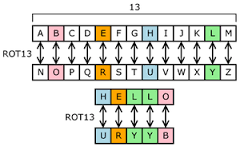
\includegraphics[scale=.8]{IMG/substitution.png}
\end{figure}
\end{frame}


\begin{frame}
\frametitle{Substitution Ciphers}

There are many different ways which we could choose our key. 
\end{frame}


\begin{frame}
\frametitle{Exercise 1: Keys to Success}

\begin{figure}

\includegraphics[scale=.7]{IMG/keys.jpeg}
\end{figure}
How many different possible keys are there?
\end{frame}

\begin{frame}
\frametitle{Keys and Keyspaces}

The size of the \textbf{keyspace} of the shift cipher is $26!$, all possible permutations of the 26 letters in the English alphabet. 
\end{frame}

\begin{frame}[fragile]
\frametitle{Coding Exercise 1: Key Generation}

First, let's use Python generate a key for the substitution cipher via a call to the function \verb|key_gen|.
\end{frame}

\begin{frame}[fragile]
\frametitle{Python Basics: The random module}

Python has a module called \verb=random= which imports some useful functions related to pseudo-random number generation. Import the module by including the following statement at the beginning of your code:
\begin{verbatim}

import random
\end{verbatim}
\end{frame}


\begin{frame}[fragile]
\frametitle{Python: The Random Module}

Access documentation for the random module here: 

\url{https://docs.python.org/3/library/random.html}
\end{frame}


\begin{frame}[fragile]
\frametitle{Python: The Random Module}

We will use the following function from the random module:
\begin{figure}
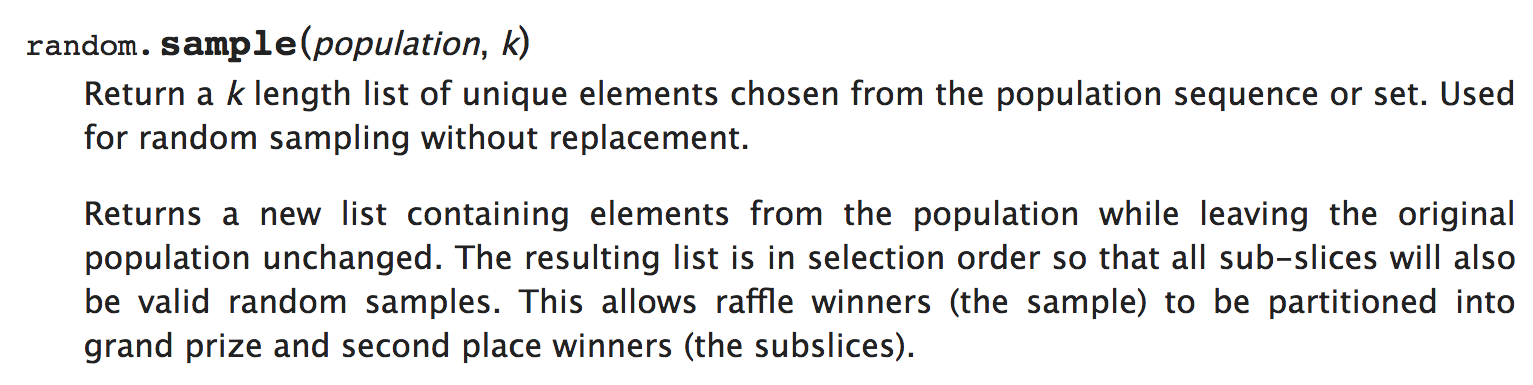
\includegraphics[scale=.4]{IMG/sample.png}
\end{figure}
\end{frame}


\begin{frame}[fragile]
\frametitle{Disclaimer on the random module}

The random module is not \emph{cryptographically secure}, a notion which will be of great importance later in the course when we study more complex encryption methods. For now, the random module will work just fine. 
\end{frame}


\begin{frame}[fragile]
\frametitle{Coding Exercise 2: Encrypt}

Next write a function called \verb|encrypt| which takes a plaintext and the key generated above as arguments and returns the ciphertext created by encrypting the plaintext under the given key using the substitution cipher. 
\end{frame}


\begin{frame}[fragile]
\frametitle{Coding Exercise 3: Decrypt}

Next write a function called \verb|decrypt| which takes a ciphertext and the key generated above as arguments and returns the plaintext corresponding to the given ciphertext.
\end{frame}


\begin{frame}
\frametitle{References}

\begin{itemize}
\item The random module: \url{https://docs.python.org/3/library/random.html}
\end{itemize}
\end{frame}
\end{document}


